\documentclass[11pt,a4paper,oneside]{article}
\usepackage{amsmath,amsthm,amsfonts,amssymb}
\usepackage{pst-eucl,pstricks,pstricks-add,multido, pst-plot}
\usepackage[utf8]{inputenc}
%\usepackage[latin1]{inputenc}
\usepackage[spanish,activeacute]{babel}
\usepackage[a4paper,margin=2.5cm]{geometry}
\usepackage{times}
\usepackage[T1]{fontenc}
\usepackage{titlesec}
\usepackage{url}
\usepackage{float}
\usepackage{cite}
\usepackage{graphicx}
\usepackage{wrapfig}
\usepackage{lipsum}
\usepackage{multicol}
\usepackage{float}
\usepackage{lmodern}
\usepackage{epstopdf}
\parindent=0mm
\usepackage{color, colortbl}
\definecolor{azul}{rgb}{0.63, 0.79, 0.95}

\newcommand*{\titleBOOK}{\begingroup
%\raggedleft
\centering
\vspace*{\baselineskip}
\vspace*{\baselineskip}
{\Huge\scshape Lecture Notes}\\[10mm]
%{\Large \includegraphics[scale=0.25]{uah.pdf}}\\[35mm]
{\Huge\scshape Non Life  \\[5mm]
Insurance} \\ [\baselineskip]
{\Large\bfseries First Draft}\\[0.3 \textheight]
{\Large Prof. Dr. Ricardo Gatto}\\
%{\large\scshape MS-PLUS, Inc.}\par
\vfill
\begin{center}
{\scshape Switzerland-Spain-Ecuador}\\
\rule{\textwidth}{0.5pt}
\end{center}
\vspace*{\baselineskip}
\endgroup}



\usepackage{Sweave}
\begin{document}
\Sconcordance{concordance:MatematicaNoVida.tex:MatematicaNoVida.Rnw:%
1 47 1 1 0 21 1 1 10 1 2 126 1 1 7 1 2 46 1}

\titleBOOK
\newpage

\tableofcontents
\newpage


\section{Individual Risk and Distributions}
A non negative random variable is called a \textbf{loss} and it its distribution a \textbf{loss distribution}.\\
$X\sim Exponential(\alpha)$ means that $X$ has density $f_X(x)=\alpha e^{-\alpha x}$ and distribution function (d.f) $F_X(x)=1-e^{-\alpha x}$ $\forall x>0$ and $\alpha>0$.\\


Let $Y=e^x$, 
\begin{align*}
F_Y(Y) &= F_X(log Y)\\
&=1-e^{\alpha log (y)}\\
&=1-y^{-\alpha}
\end{align*}
Is called the \textbf{Pareto Distribution}. If $Y$ follows a Pareto distribution, denoted  $Y\sim Pareto(\alpha)$




\begin{Schunk}
\begin{Sinput}
> x <- rnorm(100)
> y <- rnorm(100)
> plot(x,y)
\end{Sinput}
\end{Schunk}
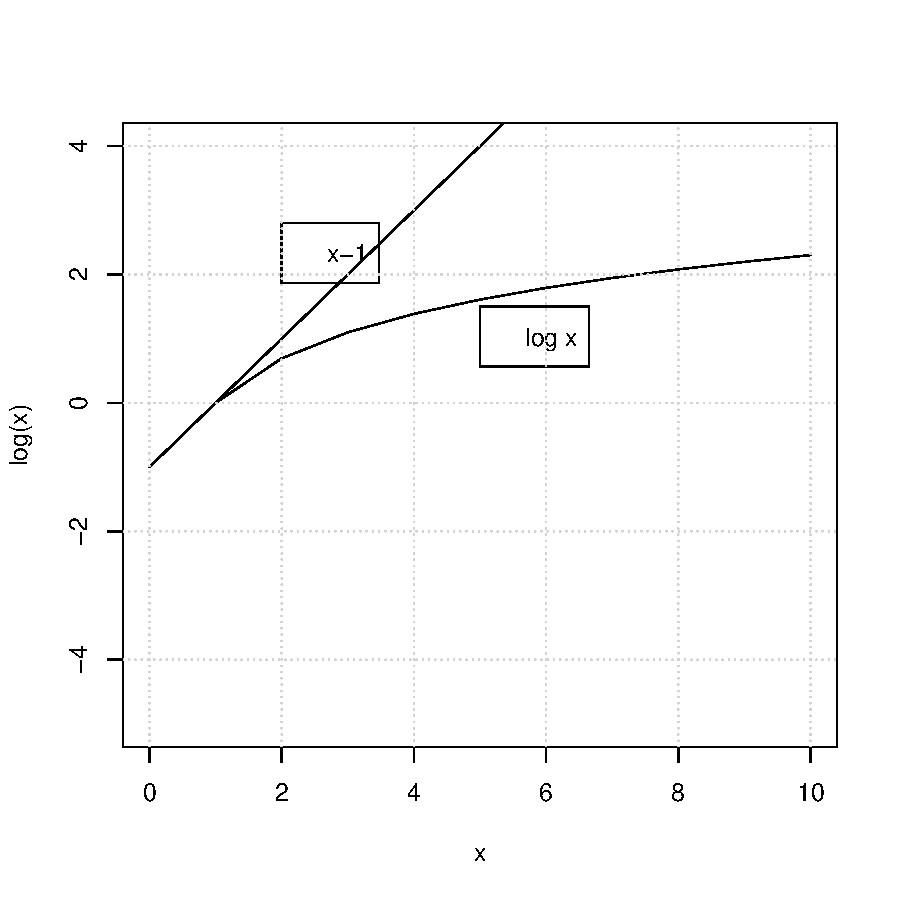
\includegraphics{MatematicaNoVida-examplePlot}

\end{document}
